\begin{flushright} {\tiny {\color{gray} pair\_q1p0stab.tex}} \end{flushright}
%~~~~~~~~~~~~~~~~~~~~~~~~~~~~~~~~~~~~~~~~~~~~~~~~~~~~~~~~~~~~~~~~~~~~~~~~~~~~~~~~~~~~~~~~~~~~~~~~~~
Much has been written about the $Q_1\times P_0$ element and the fact that it is not LBB-stable and that the pressure field contains a chequerboard mode that needs to be filtered out. 
It was the principal element used in computational geodynamics in codes such as Sopale, Citcom, Fantom, ... before being 
superseded by LBB-stable elements such as $Q_2\times Q_1$ or $Q_2\times P_{-1}$ \cite{thba21}.

Many techniques have been proposed to stabilise this element but I here focus on those which keep the number of degrees of freedom unchanged, i.e. a matrix $\C$ is added to the Stokes matrix:
\[
\left(
\begin{array}{cc}
\K & \G \\
\G^T & -\C 
\end{array}
\right)
\cdot
\left(
\begin{array}{c}
\vec{\cal V} \\
\vec{\cal P}
\end{array}
\right)
=
\left(
\begin{array}{c}
\vec{f} \\
\vec{h}
\end{array}
\right)
\]
More specifically I will focus on the pressure jump methods.

Note that in 3D the physical dimension of the $\C$ matrix is that of $h^{dim}/\eta$ (i.e. $M^{-1}L^4T$) where $h$ is the element size and $\eta$ a viscosity. The Schur complement $\SSS=\G^T\cdot \K^{-1} \cdot G$ has obviously the same dimensions with $[\G]=L^2$ and $[\K]=MT^{-1}$.

As explained in Silvester \& Kechkar \cite{sike90}: ``
The system [without the $\C$ matrix] is not strictly positive definite because of the zero coefficients on the
diagonal. This fact makes pivoting necessary when solving [the system] by direct methods and limits the applicability of almost all iterative solution techniques. What is also well-known is that for certain combinations of the approximation velocity and pressure spaces, the uniqueness of the discrete solution may not be guaranteed. This is due to the occurrence of spurious pressure modes in the pressure approximation space.''

The stability of mixed finite element methods boils down to properties of the null space of the matrix $\G$. 
An approximation is unstable if $\G \cdot \vec{\cal P} = \vec{0}$ where $\vec{\cal P}$ corresponds to some spurious pressure mode different from the constant value pressure. Note that if $\G\cdot \vec{\cal P} = \vec{0}$, then $(\vec{0},\vec{\cal P})^T$ is a null vector of  
the homogeneous system. 

The basic idea behind stabilization is to relax the incompressibility constraint in a special way so that this vector is no longer a null vector of the resulting coefficient matrix, and the discrete solutions satisfy rigorous error bounds. In other words the idea consists in regularising the system by replacing the zero block by an appropriate positive semi-definite matrix $-\C$ \cite{sike90}.
%Stabilization is applicable to any mixed approximation method. 

We will here look at so-called local and global jump methods (and their various flavours), the macro-element method, as well as the penalty method (which is not really a stabilisation method, as we will see).

\begin{itemize}
\item global jump stabilisation: 
\textcite{hufr87} (1987), \textcite{nosi98} (1998), \textcite{dowa89} (1989),
\textcite{chco01} (2001), \textcite{cao03} (2003),
\textcite{eguc03} (2003), \textcite{lica06} (2006)
\item local jump stabilisation: 
\textcite{sike90} (1990), \textcite{kesi92} (1992), \textcite{vibo92} (1992), \textcite{cao03} (2003), 
\textcite{qizh07} (2007), \textcite{chri02} (2002), \textcite{chco01} (2001),
\textcite{lisi13} (2013), \textcite{lica06} (2006)
\item stabilisation through macro-elements:
\textcite{fobo90} (1990), \textcite{leru86} (1986), \textcite{leta81} (1981)
%\item supg like stabilisation: \cite{teos00}, \cite{tezd92,hufb86}
%\item enrichment through velocity and/or pressure bubble function \cite{frol03}(only triangles)
%\item additional (normal) velocity degrees of freedom on faces \cite{fofo85}, 
%mentioned in \cite{sofo87}, \cite{fort81}.
%adding 1 dof mid-side on each face with buble function \cite{rota87}
%\item method ? : \cite{babg04},  \cite{bodg06} , \cite{bogl07}
\end{itemize}

In effect, these jump stabilisation techniques provide an a-priori filter for the weakly unstable pressure modes associated with the $Q_1\times P_0$ element. 

%Explain qh, ph notation

Consistency: in \textcite{babg04}:``we should define what we mean by a \textbf{consistent method}; perhaps
a more apt terminology would be variationally consistent. In standard usage, consistency of numerical schemes for partial differential equations requires that the pointwise
truncation error vanish as the grid size goes to zero; i.e., if one substitutes a smooth
solution of the partial differential equation into the numerical scheme, then the residual is at least o(h), where h denotes the grid size. Finite element schemes are not,
in general, consistent in this sense. However, for standard finite element methods,
sufficiently smooth exact solutions of the partial differential equations exactly satisfy
the variational equation that defines the discrete finite element equations. This is
what we mean by a consistent finite element scheme. This allows us to differentiate
between the methods we consider in this paper and methods which are not consistent
in this latter sense. For example, penalty methods for the Stokes problem are not consistent finite element methods since substitution of an exact solution into the discrete
equations leaves a residual that is proportional to the penalty parameter. Thus, we
consider only methods that do not suffer from this type of variational inconsistency.''

As explained in Elman book: ``to ensure consistency we require $\vec{1} \in null(\C)$ (this precludes the use of inconsistent 'penalty methods') and we require $\vec{p}^T\cdot \C \cdot \vec{p} >0$ for all 
spurious pressure  modes $\vec{p} \neq \vec{1}$ in $null(\G)$.''

\todo[inline]{define jump operator !! looking at sike90, I realise that I don't understand how the(ir) jump operator works in practice. Eq on page 78?}

The driving question behind all this, besides my wanting to understand these stabilisation schemes better, is the fact that 1) none of the existing publishing literature seems to address the problem of large and/or sharp viscosity contrasts/variations; 2) almost all papers deal with regular meshes and rectangular elements.

\vspace{.5cm}

%%%%%%%%%%%%%%%%%%%%%%%%%%%%%%%%%%%%%%%%%%
\paragraph{Penalty}

The conventional way of computing a regularisation matrix $\C$
is to use a penalty formulation.
In the framework presented in \textcite{sike90} (1990), the standard penalty method corresponds to the specific choice of
\begin{equation}
C(q^h,p^h)=\epsilon \int_\Omega q^h p^h \; dV = \epsilon {\M}_p
\end{equation}
with $\epsilon > 0$ and ${\M}_p$ is the pressure mass matrix. 
For a regular grid of squares with size $h$, it follows that 
\[
C_{ij}=0 \quad {\rm if} \; i\neq j
\quad\quad \text{and} \quad\quad
C_{ii}=\epsilon \int_{\Omega_i} dV = h^2 \epsilon
\]
so that the stabilisation matrix is diagonal:

\begin{center}


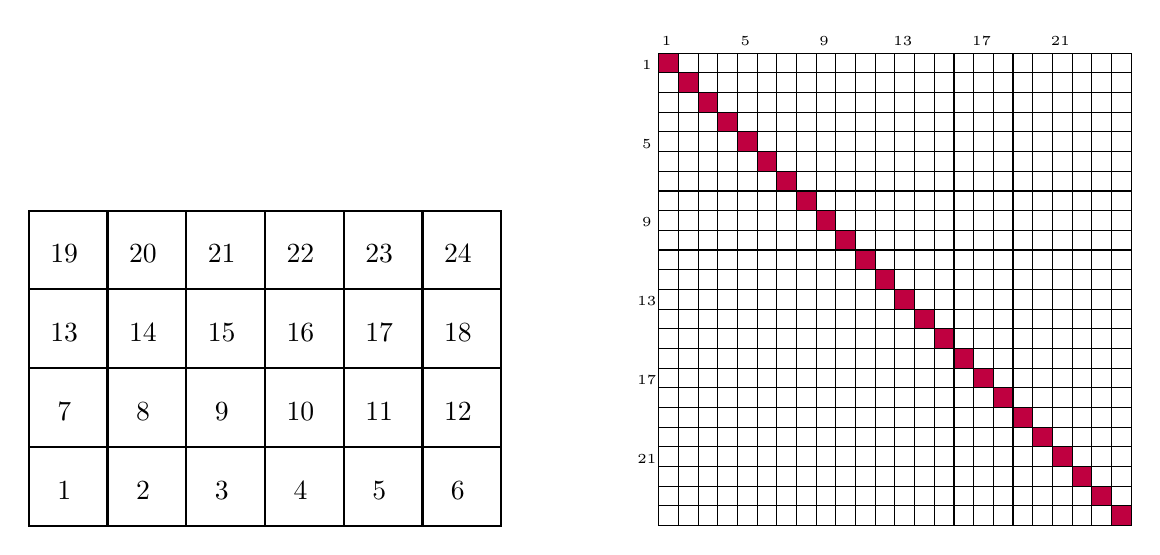
\begin{tikzpicture}
%\draw[step=0.5cm,gray,very thin] (0,0) grid (15,8); %background grid

%\draw[fill=gray!23,gray!23](0,0) rectangle (2,2);
%\draw[fill=gray!23,gray!23](2,2) rectangle (4,4);
%\draw[fill=gray!23,gray!23](4,0) rectangle (6,2);

\draw[thick] (0,0)--(6,0)--(6,4)--(0,4)--cycle;  

\draw[thick] (0,1)--(6,1);  
\draw[thick] (0,2)--(6,2);  
\draw[thick] (0,3)--(6,3);  

\draw[thick] (1,0)--(1,4);  
\draw[thick] (2,0)--(2,4);  
\draw[thick] (3,0)--(3,4);  
\draw[thick] (4,0)--(4,4);  
\draw[thick] (5,0)--(5,4);  

\node[] at (0.45,0.45) {1};
\node[] at (1.45,0.45) {2};
\node[] at (2.45,0.45) {3};
\node[] at (3.45,0.45) {4};
\node[] at (4.45,0.45) {5};
\node[] at (5.45,0.45) {6};

\node[] at (0.45,1.45) {7};
\node[] at (1.45,1.45) {8};
\node[] at (2.45,1.45) {9};
\node[] at (3.45,1.45) {10};
\node[] at (4.45,1.45) {11};
\node[] at (5.45,1.45) {12};

\node[] at (0.45,2.45) {13};
\node[] at (1.45,2.45) {14};
\node[] at (2.45,2.45) {15};
\node[] at (3.45,2.45) {16};
\node[] at (4.45,2.45) {17};
\node[] at (5.45,2.45) {18};

\node[] at (0.45,3.45) {19};
\node[] at (1.45,3.45) {20};
\node[] at (2.45,3.45) {21};
\node[] at (3.45,3.45) {22};
\node[] at (4.45,3.45) {23};
\node[] at (5.45,3.45) {24};


\node[] at (8.1,6.15) {\tiny 1};
\node[] at (9.1,6.15) {\tiny 5};
\node[] at (10.1,6.15) {\tiny 9};
\node[] at (11.1,6.15) {\tiny 13};
\node[] at (12.1,6.15) {\tiny 17};
\node[] at (13.1,6.15) {\tiny 21};

\node[] at (7.85,5.85) {\tiny 1};
\node[] at (7.85,4.85) {\tiny 5};
\node[] at (7.85,3.85) {\tiny 9};
\node[] at (7.85,2.85) {\tiny 13};
\node[] at (7.85,1.85) {\tiny 17};
\node[] at (7.85,0.85) {\tiny 21};


\draw[thin] (8,0)--(14,0)--(14,6)--(8,6)--cycle;  
\draw[step=0.25cm,black,thin] (8,0) grid (14,6); %background grid

\draw[fill=purple](8,5.75)    rectangle (8.25,6);
\draw[fill=purple](8.25,5.5)  rectangle (8.5,5.75);
\draw[fill=purple](8.5,5.25)  rectangle (8.75,5.5);
\draw[fill=purple](8.75,5)    rectangle (9,5.25);
\draw[fill=purple](9,4.75)    rectangle (9.25,5);
\draw[fill=purple](9.25,4.5)  rectangle (9.5,4.75);
\draw[fill=purple](9.5,4.25)  rectangle (9.75,4.5);
\draw[fill=purple](9.75,4)    rectangle (10,4.25);
\draw[fill=purple](10,3.75)   rectangle (10.25,4);
\draw[fill=purple](10.25,3.5) rectangle (10.5,3.75);
\draw[fill=purple](10.5,3.25) rectangle (10.75,3.5);
\draw[fill=purple](10.75,3)   rectangle (11,3.25);
\draw[fill=purple](11,2.75)   rectangle (11.25,3);
\draw[fill=purple](11.25,2.5) rectangle (11.5,2.75);
\draw[fill=purple](11.5,2.25) rectangle (11.75,2.5);
\draw[fill=purple](11.75,2)   rectangle (12,2.25);
\draw[fill=purple](12,1.75)   rectangle (12.25,2);
\draw[fill=purple](12.25,1.5) rectangle (12.5,1.75);
\draw[fill=purple](12.5,1.25) rectangle (12.75,1.5);
\draw[fill=purple](12.75,1)   rectangle (13,1.25);
\draw[fill=purple](13,0.75)   rectangle (13.25,1);
\draw[fill=purple](13.25,0.5) rectangle (13.5,0.75);
\draw[fill=purple](13.5,0.25) rectangle (13.75,0.5);
\draw[fill=purple](13.75,0)   rectangle (14,0.25);

\end{tikzpicture}
\\
{\captionfont Two-dimensional grid composed of $6\times 4$ elements
on the left and the resulting sparsity pattern of the $\C$ matrix 
on the right.}
\end{center}

In Zienkiewicz \& Taylor (Section 4.8.2) the matrix is also written as $\C = \epsilon h^2 {\bm 1} $ where ${\bm 1}$ is the unit matrix. 

It is stressed here that the penalty technique does not stabilise an  
unstable mixed method \cite{sike90}. A small penalty parameter 
means that the original problem is solved quite accurately.

See \textcite{cuss86} (1986) for some more details about the penalty method. The approach above is similar to the one presented in Section~\ref{XYZ}. The only difference is that instead of replacing the pressure in the momentum equation by $p = \lambda \vec\nabla\cdot\vec\upnu$ we keep both velocity and pressure
as unknowns and we take $\epsilon=\lambda^{-1}$. Since 
normally $\lambda >> \eta$ then $\epsilon=\lambda^{-1}$ must be small. 
As explained in Silvester \& Kechkar \cite{sike90}, 
``despite its theoretical attraction, the penalty
technique breaks down in practice because of its sensitivity to the particular choice of penalty parameter''.

The Stokes system for a single element then writes
\[
\left(
\begin{array}{cc}
\K & \G \\
\G^T & -\C 
\end{array}
\right)
\cdot
\left(
\begin{array}{c}
\vec{\cal V} \\
\vec{\cal P}
\end{array}
\right)
=
\left(
\begin{array}{cc}
\K & \G \\
\G^T & -\epsilon \M_p 
\end{array}
\right)
\cdot
\left(
\begin{array}{c}
\vec{\cal V} \\
\vec{\cal P}
\end{array}
\right)
=
\left(
\begin{array}{c}
\vec{f} \\
\vec{h}
\end{array}
\right)
\]
The second line yields
\[
\G^T \cdot \vec{\cal V} - \epsilon \M_p \cdot \vec{\cal P} = \vec{h}
\]
or, 
\[
\vec{\cal P} =\frac{1}{\epsilon} \M_p^{-1} \cdot( \G^T \cdot \vec{\cal V} -\vec{h})
\]
which can be re-introduced in the first line:
\[
\K \cdot \vec{\cal V} + \G \cdot \frac{1}{\epsilon} \M_p^{-1} \cdot( \G^T \cdot \vec{\cal V} -\vec{h}) = \vec{f}
\]
or, 
\[
\left( \K + \frac{1}{\epsilon} \G\cdot \M_p^{-1} \cdot \G^T
\right) \cdot \vec{\cal V} = \vec{f} +  \frac{1}{\epsilon}\G \cdot \M_p^{-1} \cdot \vec{h}
\]
This elimination could be carried out element by element so that one only
solves for the velocity degrees of freedom. 


- reduced integration? sike90 does not say anything about it.

- condition number explodes since $\frac{1}{\epsilon} >> \eta$

\textcite{dobo04} (2004) state: ``Penalty methods are another category of non-residual based regularizations.
They, however, differ from stabilized methods in the sense that application of a penalty does not circumvent the inf–sup condition and only serves to uncouple pressure from velocity. In
this sense, penalty methods should be viewed as solution, rather then stabilization procedures for the mixed equations.''

\vspace{.5cm}

%%%%%%%%%%%%%%%%%%%%%%%%%%%%%%%%%%%%%%%%%%
\paragraph{Global jump}

This method is explained in Silvester \& Kechkar (1990) and the authors state that it was introduced by Hughes \& Franca \cite{hufr87} in which a general theoretical framework for analysing global stabilisation techniques is presented. Using this framework, optimum rates of convergence for the $Q_1\times P_0$ method stabilised with global jumps are established.

The global jump stabilisation formulation introduces a pressure diffusion operator that perturbs the incompressibility constraint. The global jump formulation insures mass conservation in a global sense since the null space of the stabilising matrix constrains the constant-pressure vector.
However, the global jump stabilisation smears the div-free constraint over a small region, i.e., the divergence is not zero at the element level \cite{chri00}.

Consider the stabilisation term
\begin{equation}
C(q^h,p^h) 
=\beta h \sum_{s=1}^{N_s} 
\int_{\partial \Omega_s} \llbracket q^h \rrbracket  \llbracket p^h \rrbracket ds 
\end{equation}
in which $h$ is the mesh parameter (defined locally), $\llbracket . \rrbracket$ is the jump operator, and $\beta>0$ is a stabilising parameter. The summation is over {\it all} interior inter-element edges.

%from \cite{sike90}
To illustrate, consider element $9$ in the mesh consisting of equally  sized squares represented here:
\begin{center}
\input{tikz/tikz_globaljump}
\end{center}
Element 9 has four direct neighbours: 3, 8, 10, and 15.
The stabilisation term for this element involves the sum over its four neighbours:
\begin{eqnarray}
\beta h \sum_{s=1}^{4} \int_{\partial \Omega_s}[[ q^h ]]  [[p^h ]] ds
&=& \beta h^2 [ (p_9-p_3)+(p_9-p_8)+(p_9-p_{10})+(p_9-p_{15})   ]  \nn\\
&=& \beta h^2 ( 4 p_9-p_3 -p_8-p_{10} -p_{15})  \nn
\end{eqnarray}
The integral along each edge is simply the pressure difference across the edge 
multiplied by the edge surface/length which happens to be constant in this case.
This means that the in the matrix $\C$, there will be entries on the $9^{th}$
line at columns 3, 8, 10, and 15. 

Be careful, let us now turn to element 6: it has 2 neighbours (5 and 12), so that
the stabilisation term for this element involves the sum over its two neighbours:
\begin{eqnarray}
 \beta h^2 [ (p_6-p_5)+(p_6-p_{12})  ]  
&=& \beta h^2 ( 2 p_6-p_5 -p_{12} )  \nn
\end{eqnarray}

And looking now at element 23: it has three neighbours (17, 22, and 24), so that 
the stabilisation term for this element involves the sum over its three neighbours:
\begin{eqnarray}
\beta h^2 [ (p_{23}-p_{17})+(p_{23}-p_{22}) +(p_{23}-p_{24})  ] 
&=& \beta h^2 ( 3 p_{23}-p_{17} -p_{22} - p_{24} )  \nn
\end{eqnarray}

The resulting assembled $\C$ matrix is shown here:
\begin{center}

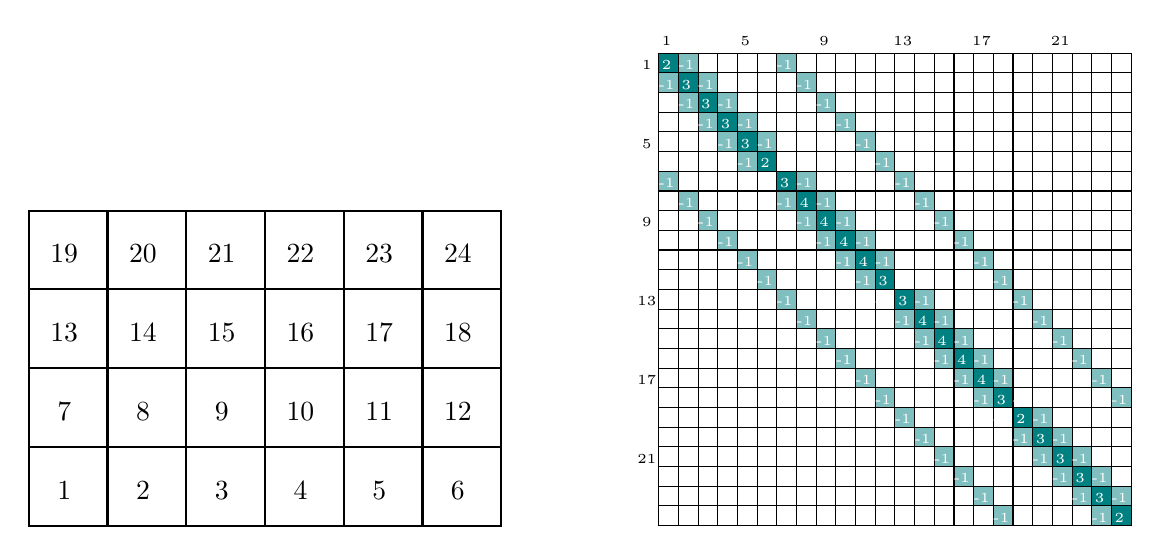
\begin{tikzpicture}
%\draw[step=0.5cm,gray,very thin] (0,0) grid (15,8); %background grid

%\draw[fill=gray!23,gray!23](0,0) rectangle (2,2);
%\draw[fill=gray!23,gray!23](2,2) rectangle (4,4);
%\draw[fill=gray!23,gray!23](4,0) rectangle (6,2);

\draw[thick] (0,0)--(6,0)--(6,4)--(0,4)--cycle;  

\draw[thick] (0,1)--(6,1);  
\draw[thick] (0,2)--(6,2);  
\draw[thick] (0,3)--(6,3);  

\draw[thick] (1,0)--(1,4);  
\draw[thick] (2,0)--(2,4);  
\draw[thick] (3,0)--(3,4);  
\draw[thick] (4,0)--(4,4);  
\draw[thick] (5,0)--(5,4);  

\node[] at (0.45,0.45) {1};
\node[] at (1.45,0.45) {2};
\node[] at (2.45,0.45) {3};
\node[] at (3.45,0.45) {4};
\node[] at (4.45,0.45) {5};
\node[] at (5.45,0.45) {6};

\node[] at (0.45,1.45) {7};
\node[] at (1.45,1.45) {8};
\node[] at (2.45,1.45) {9};
\node[] at (3.45,1.45) {10};
\node[] at (4.45,1.45) {11};
\node[] at (5.45,1.45) {12};

\node[] at (0.45,2.45) {13};
\node[] at (1.45,2.45) {14};
\node[] at (2.45,2.45) {15};
\node[] at (3.45,2.45) {16};
\node[] at (4.45,2.45) {17};
\node[] at (5.45,2.45) {18};

\node[] at (0.45,3.45) {19};
\node[] at (1.45,3.45) {20};
\node[] at (2.45,3.45) {21};
\node[] at (3.45,3.45) {22};
\node[] at (4.45,3.45) {23};
\node[] at (5.45,3.45) {24};

\node[] at (8.1,6.15) {\tiny 1};
\node[] at (9.1,6.15) {\tiny 5};
\node[] at (10.1,6.15) {\tiny 9};
\node[] at (11.1,6.15) {\tiny 13};
\node[] at (12.1,6.15) {\tiny 17};
\node[] at (13.1,6.15) {\tiny 21};

\node[] at (7.85,5.85) {\tiny 1};
\node[] at (7.85,4.85) {\tiny 5};
\node[] at (7.85,3.85) {\tiny 9};
\node[] at (7.85,2.85) {\tiny 13};
\node[] at (7.85,1.85) {\tiny 17};
\node[] at (7.85,0.85) {\tiny 21};


\draw[thin] (8,0)--(14,0)--(14,6)--(8,6)--cycle;  
\draw[step=0.25cm,black,thin] (8,0) grid (14,6); %background grid


%1
\draw[fill=teal](8,5.75)    rectangle (8.25,6);
\draw[fill=teal!50](8.25,5.75) rectangle (8.5,6);
\draw[fill=teal!50](9.5,5.75)  rectangle (9.75,6);
\node[white,font=\fontsize{3}{3.5}\selectfont] at (8.1,5.85){2};
\node[white,font=\fontsize{3}{3.5}\selectfont] at (8.35,5.85){-1};
\node[white,font=\fontsize{3}{3.5}\selectfont] at (9.6,5.85){-1};

%2
\draw[fill=teal](8.25,5.5)  rectangle (8.5,5.75);
\draw[fill=teal!50](9.75,5.5)  rectangle (10,5.75);
\draw[fill=teal!50](8,5.5) rectangle (8.25,5.75);
\draw[fill=teal!50](8.5,5.5) rectangle (8.75,5.75);
\node[white,font=\fontsize{3}{3.5}\selectfont] at (8.35,5.6){3};
\node[white,font=\fontsize{3}{3.5}\selectfont] at (9.85,5.6){-1};
\node[white,font=\fontsize{3}{3.5}\selectfont] at (8.6,5.6){-1};
\node[white,font=\fontsize{3}{3.5}\selectfont] at (8.1,5.6){-1};

%3
\draw[fill=teal](8.5,5.25)  rectangle (8.75,5.5);
\draw[fill=teal!50](10,5.25)   rectangle (10.25,5.5);
\draw[fill=teal!50](8.25,5.25) rectangle (8.5,5.5);
\draw[fill=teal!50](8.75,5.25) rectangle (9,5.5);
\node[white,font=\fontsize{3}{3.5}\selectfont] at (8.6,5.35){3};
\node[white,font=\fontsize{3}{3.5}\selectfont] at (10.1,5.35){-1};
\node[white,font=\fontsize{3}{3.5}\selectfont] at (8.85,5.35){-1};
\node[white,font=\fontsize{3}{3.5}\selectfont] at (8.35,5.35){-1};

%4
\draw[fill=teal](8.75,5)    rectangle (9,5.25);
\draw[fill=teal!50](10.25,5)   rectangle (10.5,5.25);
\draw[fill=teal!50](8.5,5) rectangle (8.75,5.25);
\draw[fill=teal!50](9,5) rectangle (9.25,5.25);
\node[white,font=\fontsize{3}{3.5}\selectfont] at (8.85,5.1){3};
\node[white,font=\fontsize{3}{3.5}\selectfont] at (10.35,5.1){-1};
\node[white,font=\fontsize{3}{3.5}\selectfont] at (9.1,5.1){-1};
\node[white,font=\fontsize{3}{3.5}\selectfont] at (8.6,5.1){-1};

%5
\draw[fill=teal](9,4.75)    rectangle (9.25,5);
\draw[fill=teal!50](10.5,4.75) rectangle (10.75,5);
\draw[fill=teal!50](8.75,4.75) rectangle (9,5);
\draw[fill=teal!50](9.25,4.75) rectangle (9.5,5);
\node[white,font=\fontsize{3}{3.5}\selectfont] at (9.1,4.85){3};
\node[white,font=\fontsize{3}{3.5}\selectfont] at (10.6,4.85){-1};
\node[white,font=\fontsize{3}{3.5}\selectfont] at (9.35,4.85){-1};
\node[white,font=\fontsize{3}{3.5}\selectfont] at (8.85,4.85){-1};

%6
\draw[fill=teal](9.25,4.5)  rectangle (9.5,4.75);
\draw[fill=teal!50](10.75,4.5) rectangle (11,4.75);
\draw[fill=teal!50](9,4.5) rectangle (9.25,4.75);
%\draw[fill=teal!50](9.5,4.5) rectangle (9.75,4.75);
\node[white,font=\fontsize{3}{3.5}\selectfont] at (9.35,4.6){2};
\node[white,font=\fontsize{3}{3.5}\selectfont] at (9.6,4.6){-1};
\node[white,font=\fontsize{3}{3.5}\selectfont] at (10.85,4.6){-1};
\node[white,font=\fontsize{3}{3.5}\selectfont] at (9.1,4.6){-1};

%7
\draw[fill=teal](9.5,4.25)  rectangle (9.75,4.5);
\draw[fill=teal!50](11,4.25)   rectangle (11.25,4.5);
%\draw[fill=teal!50](9.25,4.25) rectangle (9.5,4.5);
\draw[fill=teal!50](9.75,4.25) rectangle (10,4.5);
\draw[fill=teal!50](8,4.25)   rectangle (8.25,4.5);
\node[white,font=\fontsize{3}{3.5}\selectfont] at (9.6,4.35){3};
\node[white,font=\fontsize{3}{3.5}\selectfont] at (9.85,4.35){-1};
\node[white,font=\fontsize{3}{3.5}\selectfont] at (11.1,4.35){-1};
%\node[white,font=\fontsize{3}{3.5}\selectfont] at (9.35,4.35){-1};
\node[white,font=\fontsize{3}{3.5}\selectfont] at (8.1,4.35){-1};

%8
\draw[fill=teal](9.75,4)    rectangle (10,4.25);
\draw[fill=teal!50](11.25,4)   rectangle (11.5,4.25);
\draw[fill=teal!50](9.5,4) rectangle (9.75,4.25);
\draw[fill=teal!50](10,4) rectangle (10.25,4.25);
\draw[fill=teal!50](8.25,4)   rectangle (8.5,4.25);
\node[white,font=\fontsize{3}{3.5}\selectfont] at (9.85,4.1){4};
\node[white,font=\fontsize{3}{3.5}\selectfont] at (11.35,4.1){-1};
\node[white,font=\fontsize{3}{3.5}\selectfont] at (10.1,4.1){-1};
\node[white,font=\fontsize{3}{3.5}\selectfont] at (9.6,4.1){-1};
\node[white,font=\fontsize{3}{3.5}\selectfont] at (8.35,4.1){-1};

%9
\draw[fill=teal](10,3.75)   rectangle (10.25,4);
\draw[fill=teal!50](11.5,3.75) rectangle (11.75,4);
\draw[fill=teal!50](9.75,3.75) rectangle (10,4);
\draw[fill=teal!50](10.25,3.75) rectangle (10.5,4);
\draw[fill=teal!50](8.5,3.75) rectangle (8.75,4);
\node[white,font=\fontsize{3}{3.5}\selectfont] at (10.1,3.85){4};
\node[white,font=\fontsize{3}{3.5}\selectfont] at (11.6,3.85){-1};
\node[white,font=\fontsize{3}{3.5}\selectfont] at (10.35,3.85){-1};
\node[white,font=\fontsize{3}{3.5}\selectfont] at (9.85,3.85){-1};
\node[white,font=\fontsize{3}{3.5}\selectfont] at (8.6,3.85){-1};

%10
\draw[fill=teal](10.25,3.5) rectangle (10.5,3.75);
\draw[fill=teal!50](11.75,3.5) rectangle (12,3.75);
\draw[fill=teal!50](10,3.5) rectangle (10.25,3.75);
\draw[fill=teal!50](10.5,3.5) rectangle (10.75,3.75);
\draw[fill=teal!50](8.75,3.5) rectangle (9,3.75);
\node[white,font=\fontsize{3}{3.5}\selectfont] at (10.35,3.6){4};
\node[white,font=\fontsize{3}{3.5}\selectfont] at (11.85,3.6){-1};
\node[white,font=\fontsize{3}{3.5}\selectfont] at (10.6,3.6){-1};
\node[white,font=\fontsize{3}{3.5}\selectfont] at (10.1,3.6){-1};
\node[white,font=\fontsize{3}{3.5}\selectfont] at (8.85,3.6){-1};

%11
\draw[fill=teal](10.5,3.25) rectangle (10.75,3.5);
\draw[fill=teal!50](12,3.25)   rectangle (12.25,3.5);
\draw[fill=teal!50](10.25,3.25) rectangle (10.5,3.5);
\draw[fill=teal!50](10.75,3.25) rectangle (11,3.5);
\draw[fill=teal!50](9,3.25) rectangle (9.25,3.5);
\node[white,font=\fontsize{3}{3.5}\selectfont] at (10.6,3.35){4};
\node[white,font=\fontsize{3}{3.5}\selectfont] at (12.1,3.35){-1};
\node[white,font=\fontsize{3}{3.5}\selectfont] at (10.85,3.35){-1};
\node[white,font=\fontsize{3}{3.5}\selectfont] at (10.35,3.35){-1};
\node[white,font=\fontsize{3}{3.5}\selectfont] at (9.1,3.35){-1};

%12
\draw[fill=teal](10.75,3)   rectangle (11,3.25);
\draw[fill=teal!50](12.25,3)   rectangle (12.5,3.25);
\draw[fill=teal!50](10.5,3) rectangle (10.75,3.25);
%\draw[fill=teal!50](11,3) rectangle (11.25,3.25);
\draw[fill=teal!50](9.25,3) rectangle (9.5,3.25);
\node[white,font=\fontsize{3}{3.5}\selectfont] at (10.85,3.1){3};
\node[white,font=\fontsize{3}{3.5}\selectfont] at (12.35,3.1){-1};
%\node[white,font=\fontsize{3}{3.5}\selectfont] at (11.1,3.1){-1};
\node[white,font=\fontsize{3}{3.5}\selectfont] at (10.6,3.1){-1};
\node[white,font=\fontsize{3}{3.5}\selectfont] at (9.35,3.1){-1};

%13
\draw[fill=teal](11,2.75)   rectangle (11.25,3);
\draw[fill=teal!50](12.5,2.75) rectangle (12.75,3);
%\draw[fill=teal!50](10.75,2.75) rectangle (11,3);
\draw[fill=teal!50](11.25,2.75) rectangle (11.5,3);
\draw[fill=teal!50](9.5,2.75) rectangle (9.75,3);
\node[white,font=\fontsize{3}{3.5}\selectfont] at (11.1,2.85){3};
\node[white,font=\fontsize{3}{3.5}\selectfont] at (12.6,2.85){-1};
\node[white,font=\fontsize{3}{3.5}\selectfont] at (11.35,2.85){-1};
\node[white,font=\fontsize{3}{3.5}\selectfont] at (10.85,2.85){-1};
\node[white,font=\fontsize{3}{3.5}\selectfont] at (9.6,2.85){-1};

%14
\draw[fill=teal](11.25,2.5) rectangle (11.5,2.75);
\draw[fill=teal!50](12.75,2.5) rectangle (13,2.75);
\draw[fill=teal!50](11,2.5) rectangle (11.25,2.75);
\draw[fill=teal!50](11.5,2.5) rectangle (11.75,2.75);
\draw[fill=teal!50](9.75,2.5) rectangle (10,2.75);
\node[white,font=\fontsize{3}{3.5}\selectfont] at (11.35,2.6){4};
\node[white,font=\fontsize{3}{3.5}\selectfont] at (12.85,2.6){-1};
\node[white,font=\fontsize{3}{3.5}\selectfont] at (11.6,2.6){-1};
\node[white,font=\fontsize{3}{3.5}\selectfont] at (11.1,2.6){-1};
\node[white,font=\fontsize{3}{3.5}\selectfont] at (9.85,2.6){-1};

%15
\draw[fill=teal](11.5,2.25) rectangle (11.75,2.5);
\draw[fill=teal!50](13,2.25)   rectangle (13.25,2.5);
\draw[fill=teal!50](11.25,2.25) rectangle (11.5,2.5);
\draw[fill=teal!50](11.75,2.25) rectangle (12,2.5);
\draw[fill=teal!50](10,2.25) rectangle (10.25,2.5);
\node[white,font=\fontsize{3}{3.5}\selectfont] at (11.6,2.35){4};
\node[white,font=\fontsize{3}{3.5}\selectfont] at (13.1,2.35){-1};
\node[white,font=\fontsize{3}{3.5}\selectfont] at (11.85,2.35){-1};
\node[white,font=\fontsize{3}{3.5}\selectfont] at (11.35,2.35){-1};
\node[white,font=\fontsize{3}{3.5}\selectfont] at (10.1,2.35){-1};

%16
\draw[fill=teal](11.75,2)   rectangle (12,2.25);
\draw[fill=teal!50](13.25,2)   rectangle (13.5,2.25);
\draw[fill=teal!50](11.5,2) rectangle (11.75,2.25);
\draw[fill=teal!50](12,2) rectangle (12.25,2.25);
\draw[fill=teal!50](10.25,2) rectangle (10.5,2.25);
\node[white,font=\fontsize{3}{3.5}\selectfont] at (11.85,2.1){4};
\node[white,font=\fontsize{3}{3.5}\selectfont] at (13.35,2.1){-1};
\node[white,font=\fontsize{3}{3.5}\selectfont] at (12.1,2.1){-1};
\node[white,font=\fontsize{3}{3.5}\selectfont] at (11.6,2.1){-1};
\node[white,font=\fontsize{3}{3.5}\selectfont] at (10.35,2.1){-1};

%17
\draw[fill=teal](12,1.75)   rectangle (12.25,2);
\draw[fill=teal!50](13.5,1.75) rectangle (13.75,2);
\draw[fill=teal!50](11.75,1.75) rectangle (12,2);
\draw[fill=teal!50](12.25,1.75) rectangle (12.5,2);
\draw[fill=teal!50](10.5,1.75) rectangle (10.75,2);
\node[white,font=\fontsize{3}{3.5}\selectfont] at (12.1,1.85){4};
\node[white,font=\fontsize{3}{3.5}\selectfont] at (13.6,1.85){-1};
\node[white,font=\fontsize{3}{3.5}\selectfont] at (12.35,1.85){-1};
\node[white,font=\fontsize{3}{3.5}\selectfont] at (11.85,1.85){-1};
\node[white,font=\fontsize{3}{3.5}\selectfont] at (10.6,1.85){-1};

%18
\draw[fill=teal](12.25,1.5) rectangle (12.5,1.75);
\draw[fill=teal!50](13.75,1.5) rectangle (14,1.75);
\draw[fill=teal!50](12,1.5) rectangle (12.25,1.75);
%\draw[fill=teal!50](12.5,1.5) rectangle (12.75,1.75);
\draw[fill=teal!50](10.75,1.5) rectangle (11,1.75);
\node[white,font=\fontsize{3}{3.5}\selectfont] at (12.35,1.6){3};
\node[white,font=\fontsize{3}{3.5}\selectfont] at (13.85,1.6){-1};
\node[white,font=\fontsize{3}{3.5}\selectfont] at (12.6,1.6){-1};
\node[white,font=\fontsize{3}{3.5}\selectfont] at (12.1,1.6){-1};
\node[white,font=\fontsize{3}{3.5}\selectfont] at (10.85,1.6){-1};

%19
\draw[fill=teal](12.5,1.25) rectangle (12.75,1.5);
%\draw[fill=teal!50](12.25,1.25) rectangle (12.5,1.5);
\draw[fill=teal!50](12.75,1.25) rectangle (13,1.5);
\draw[fill=teal!50](11,1.25) rectangle (11.25,1.5);
\node[white,font=\fontsize{3}{3.5}\selectfont] at (12.6,1.35){2};
\node[white,font=\fontsize{3}{3.5}\selectfont] at (12.85,1.35){-1};
\node[white,font=\fontsize{3}{3.5}\selectfont] at (12.35,1.35){-1};
\node[white,font=\fontsize{3}{3.5}\selectfont] at (11.1,1.35){-1};

%20
\draw[fill=teal](12.75,1)   rectangle (13,1.25);
\draw[fill=teal!50](12.5,1) rectangle (12.75,1.25);
\draw[fill=teal!50](13,1) rectangle (13.25,1.25);
\draw[fill=teal!50](11.25,1) rectangle (11.5,1.25);
\node[white,font=\fontsize{3}{3.5}\selectfont] at (12.85,1.1){3};
\node[white,font=\fontsize{3}{3.5}\selectfont] at (13.1,1.1){-1};
\node[white,font=\fontsize{3}{3.5}\selectfont] at (12.6,1.1){-1};
\node[white,font=\fontsize{3}{3.5}\selectfont] at (11.35,1.1){-1};

%21
\draw[fill=teal](13,0.75)   rectangle (13.25,1);
\draw[fill=teal!50](12.75,0.75) rectangle (13,1);
\draw[fill=teal!50](13.25,0.75) rectangle (13.5,1);
\draw[fill=teal!50](11.5,0.75) rectangle (11.75,1);
\node[white,font=\fontsize{3}{3.5}\selectfont] at (13.1,0.85){3};
\node[white,font=\fontsize{3}{3.5}\selectfont] at (13.35,0.85){-1};
\node[white,font=\fontsize{3}{3.5}\selectfont] at (12.85,0.85){-1};
\node[white,font=\fontsize{3}{3.5}\selectfont] at (11.6,0.85){-1};

%22
\draw[fill=teal](13.25,0.5) rectangle (13.5,0.75);
\draw[fill=teal!50](13,0.5) rectangle (13.25,0.75);
\draw[fill=teal!50](13.5,0.5) rectangle (13.75,0.75);
\draw[fill=teal!50](11.75,0.5) rectangle (12,0.75);
\node[white,font=\fontsize{3}{3.5}\selectfont] at (13.35,0.6){3};
\node[white,font=\fontsize{3}{3.5}\selectfont] at (13.6,0.6){-1};
\node[white,font=\fontsize{3}{3.5}\selectfont] at (13.1,0.6){-1};
\node[white,font=\fontsize{3}{3.5}\selectfont] at (11.85,0.6){-1};

%23
\draw[fill=teal](13.5,0.25) rectangle (13.75,0.5);
\draw[fill=teal!50](13.25,0.25) rectangle (13.5,0.5);
\draw[fill=teal!50](13.75,0.25) rectangle (14,0.5);
\draw[fill=teal!50](12,0.25) rectangle (12.25,0.5);
\node[white,font=\fontsize{3}{3.5}\selectfont] at (13.6,0.35){3};
\node[white,font=\fontsize{3}{3.5}\selectfont] at (13.85,0.35){-1};
\node[white,font=\fontsize{3}{3.5}\selectfont] at (13.35,0.35){-1};
\node[white,font=\fontsize{3}{3.5}\selectfont] at (12.1,0.35){-1};

%24
\draw[fill=teal](13.75,0)   rectangle (14,0.25);
\draw[fill=teal!50](13.5,0) rectangle (13.75,0.25);
\draw[fill=teal!50](12.25,0) rectangle (12.5,0.25);
\node[white,font=\fontsize{3}{3.5}\selectfont] at (13.85,0.1){2};
\node[white,font=\fontsize{3}{3.5}\selectfont] at (13.6,0.1){-1};
\node[white,font=\fontsize{3}{3.5}\selectfont] at (12.35,0.1){-1};


\end{tikzpicture}

\end{center}
As stated in \cite{sike90}, ``for a natural numbering strategy the stabilisation matrix C is pentadiagonal''.

The global jump stabilisation is effective in practice, although a careful choice of the parameter $\beta$ is required in order to prevent a loss of accuracy in the solution. According to \textcite{sike90} the only other deficiency is the fact that the global nature of the jump terms makes the method awkward to implement into existing codes \footnote{I don't understand this remark}.

Let us now consider the following chequerboard pressure mode:
\begin{center}
\begin{flushright} {\tiny {\color{gray} (tikz\_chequerboard.tex)}} \end{flushright}
%~~~~~~~~~~~~~~~~~~~~~~~~~~~~~~~~~~~~~~~~~~~~~~~~~~~~~~~~~~~~~~~~~~~~~~~~~~~~~~~~~~~~~~~~~~~~~~~~~~

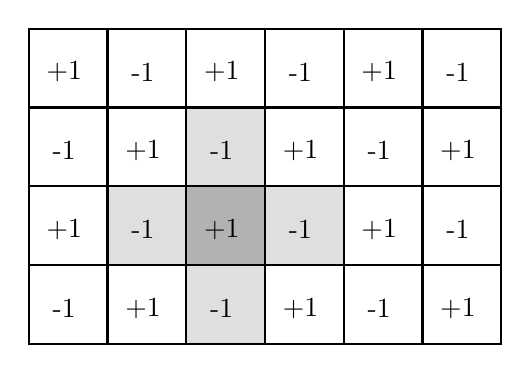
\begin{tikzpicture}
%\draw[step=0.5cm,gray,very thin] (0,0) grid (6,4); %background grid

\draw[fill=gray!60,gray!60](2,1) rectangle (3,2);
\draw[fill=gray!25,gray!25](2,0) rectangle (3,1);
\draw[fill=gray!25,gray!25](2,2) rectangle (3,3);
\draw[fill=gray!25,gray!25](1,1) rectangle (2,2);
\draw[fill=gray!25,gray!25](3,1) rectangle (4,2);

\draw[thick] (0,0)--(6,0)--(6,4)--(0,4)--cycle;  

\draw[thick] (0,1)--(6,1);  
\draw[thick] (0,2)--(6,2);  
\draw[thick] (0,3)--(6,3);  

\draw[thick] (1,0)--(1,4);  
\draw[thick] (2,0)--(2,4);  
\draw[thick] (3,0)--(3,4);  
\draw[thick] (4,0)--(4,4);  
\draw[thick] (5,0)--(5,4);  

\node[] at (0.45,0.45) {-1};
\node[] at (1.45,0.45) {+1};
\node[] at (2.45,0.45) {-1};
\node[] at (3.45,0.45) {+1};
\node[] at (4.45,0.45) {-1};
\node[] at (5.45,0.45) {+1};

\node[] at (0.45,1.45) {+1};
\node[] at (1.45,1.45) {-1};
\node[] at (2.45,1.45) {+1};
\node[] at (3.45,1.45) {-1};
\node[] at (4.45,1.45) {+1};
\node[] at (5.45,1.45) {-1};

\node[] at (0.45,2.45) {-1};
\node[] at (1.45,2.45) {+1};
\node[] at (2.45,2.45) {-1};
\node[] at (3.45,2.45) {+1};
\node[] at (4.45,2.45) {-1};
\node[] at (5.45,2.45) {+1};

\node[] at (0.45,3.45) {+1};
\node[] at (1.45,3.45) {-1};
\node[] at (2.45,3.45) {+1};
\node[] at (3.45,3.45) {-1};
\node[] at (4.45,3.45) {+1};
\node[] at (5.45,3.45) {-1};

\end{tikzpicture}



\end{center}
We find 
\[
\beta h^2 ( 4 p_9-p_3 -p_8-p_{10} -p_{15})  
=
\beta h^2 ( 4 \cdot (+1)-(-1) -(-1)-(-1) -(-1))  
= 8 \beta h^2 \ne 0
\]

\begin{remark}
In \textcite{cao03} (2003) the parameter $\beta$ is set to 1.
\end{remark}

\begin{remark}
Note that this approach is somewhat linked to the idea of a pressure smoother via a discrete  Laplace\footnote{\url{http://en.wikipedia.org/wiki/Discrete_Laplace_operator}}:
The Discrete Laplace operator is often used in image processing e.g. in edge detection and motion estimation applications. The discrete Laplacian is defined as the sum of the second derivatives Laplace
and calculated as sum of differences over the nearest neighbours of the central pixel. Here is an example of a 2D filter and it is of course similar in nature to the Global
stabilisation stensil matrix:
\[
D^{(1)}=
\left[
\begin{array}{ccc}
0 &-1 &0\\
-1 &+4 &-1\\
0 &-1 &0
\end{array}
\right]
\]
Note that other filters can also be found although we will not use them here in this context:
\[
D^{(2)}=
\left[
\begin{array}{ccc}
-0.5 &-1 &-0.5\\
-1 &+6 &-1\\
-0.5 &-1 &-0.5
\end{array}
\right]
\quad\quad\quad
D^{(3)}=
\left[
\begin{array}{ccc}
-1 &-1 &-1\\
-1 &+8 &-1\\
-1 &-1 &-1
\end{array}
\right]
\quad\quad\quad
D^{(4)}=
\left[
\begin{array}{ccc}
1 & -2 & 1 \\
-2 & 4 & -2 \\
1 & -2 & 1 \\
\end{array}
\right]
\]
\end{remark}    

Eguchi (2003) adds a linear form to the global stab $\C$ to suppress the pressure nullspace.

\vspace{.5cm}

%%%%%%%%%%%%%%%%%%%%%%%%%%%%%%%%%%%%%%%%%%%%%%%%%%%%%%%%%
\paragraph{Local jump}

According to \textcite{sike90}, the deficiencies of the global jump method can be overcome by a straightforward modification. Assume that the elements in can now be assembled into $N_m$ disjoint macro-elements
of $2\times 2$ elements, as shown in grey on the following figure:

\begin{center}
\begin{flushright} {\tiny {\color{gray} (tikz\_localjump.tex)}} \end{flushright}
%~~~~~~~~~~~~~~~~~~~~~~~~~~~~~~~~~~~~~~~~~~~~~~~~~~~~~~~~~~~~~~~~~~~~~~~~~~~~~~~~~~~~~~~~~~~~~~~~~~


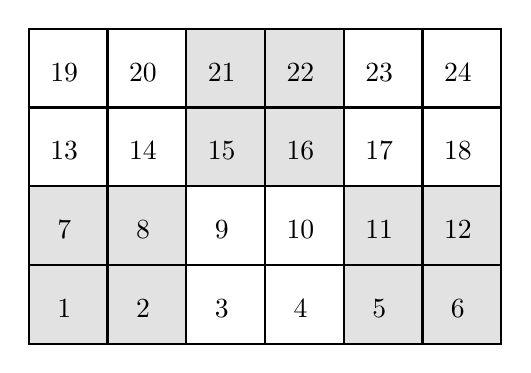
\begin{tikzpicture}
%\draw[step=0.5cm,gray,very thin] (0,0) grid (6,4); %background grid

\draw[fill=gray!23,gray!23](0,0) rectangle (2,2);
\draw[fill=gray!23,gray!23](2,2) rectangle (4,4);
\draw[fill=gray!23,gray!23](4,0) rectangle (6,2);

\draw[thick] (0,0)--(6,0)--(6,4)--(0,4)--cycle;  

\draw[thick] (0,1)--(6,1);  
\draw[thick] (0,2)--(6,2);  
\draw[thick] (0,3)--(6,3);  

\draw[thick] (1,0)--(1,4);  
\draw[thick] (2,0)--(2,4);  
\draw[thick] (3,0)--(3,4);  
\draw[thick] (4,0)--(4,4);  
\draw[thick] (5,0)--(5,4);  

\node[] at (0.45,0.45) {1};
\node[] at (1.45,0.45) {2};
\node[] at (2.45,0.45) {3};
\node[] at (3.45,0.45) {4};
\node[] at (4.45,0.45) {5};
\node[] at (5.45,0.45) {6};

\node[] at (0.45,1.45) {7};
\node[] at (1.45,1.45) {8};
\node[] at (2.45,1.45) {9};
\node[] at (3.45,1.45) {10};
\node[] at (4.45,1.45) {11};
\node[] at (5.45,1.45) {12};

\node[] at (0.45,2.45) {13};
\node[] at (1.45,2.45) {14};
\node[] at (2.45,2.45) {15};
\node[] at (3.45,2.45) {16};
\node[] at (4.45,2.45) {17};
\node[] at (5.45,2.45) {18};

\node[] at (0.45,3.45) {19};
\node[] at (1.45,3.45) {20};
\node[] at (2.45,3.45) {21};
\node[] at (3.45,3.45) {22};
\node[] at (4.45,3.45) {23};
\node[] at (5.45,3.45) {24};

\end{tikzpicture}


\end{center}

Consider now the bilinear form given by
\[
C(q^h,p^h) = \beta h \sum_{m=1}^{N_m} \sum_{i=1}^4 \int_{\partial \Omega_m} \llbracket q^h \rrbracket  \llbracket p^h \rrbracket ds
\]
where the first summation is over all $2\times 2$ macroelements,
and the second summation runs over all inter element edges strictly within each macroelelement.

The form of the stabilisation matrix $\C$ is similar to that above except that there is now a local basis.

For instance, considering again element 9, it now belongs to the second macro-element and therefore only 'sees' neighbours 3 and 10.
The resulting $\C$ matrix is shown on the figure here after and
its structure is obviously different than in the global stabilisation case, albeit also pentadiagonal.

\begin{center}
\input{tikz/tikz_q1p0stab_local}
\end{center}

\begin{remark}
Obviously, one could re-number the elements so that matrix $\C$
is block diagonal: macroelement 1 would contain elements 1,2,3,4, macroelement 2 would contain elements 5,6,7,8, etc ... 
\end{remark}

According to \textcite{sike90} or \textcite{chke20}, the advantages of this local method over the global jump
formulation are:
\begin{enumerate}
\item implementation is more straightforward because for assembly purposes each $2\times 2$ block of elements can be treated as a single macroelement \footnote{same here, not sure what they mean by this}
\item mass is conserved locally (over a macroelement), using the global jump formulation mass is only conserved globally
\item robustness is improved in the sense that the discrete velocity solution is less sensitive to the magnitude of $\beta$, the influence of the stabilisation matrix being localised (will need to be tested numerically!). 
\end{enumerate}

\begin{remark}
The globally stabilised formulation corresponds to the
extreme case of a local stabilisation based on a single macro-element \cite{grsa}.
\end{remark}

One of the features of the local stabilisation is that if the discrete incompressibility constraints are added together then the jump terms sum to zero in each macro element.
Indeed, let us consider the following macro element:

\begin{center}
\input{tikz/tikz_macro}
\end{center}

The corresponding matrix (making abstraction of the $\beta$ term) writes:
\[
h^2
\left(
\begin{array}{cccc}
2 & -1 & -1 &0 \\
-1 & 2 & 0 & -1 \\
-1 & 0 & 2 & -1 \\
0 & -1 & -1 & 2
\end{array}
\right)
\left(
\begin{array}{c}
p_1 \\ p_2 \\ p_3 \\ p_4
\end{array}
\right)
\]
and the row/column sum of its entries is always null. Also, 
$\C$ is obviously positive semi-definite \cite{sike90}.

Gresho \& Sani \cite{grsa} state:``
This is crucially important to the success of the method since it implies that the local incompressibility of the $Q_1\times P_0$ method is retained after stabilisation (albeit over macro-elements).
It also suggests that a good strategy when constructing the partition
is to form macro-elements containing as few elements as possible.
Once a suitable macro-element partitioning has been formed, the local stabilisation matrices can be calculated by running through the component elements, summing jump contributions corresponding to the internal edges.''

If one now considers the following irregular macro-element,
\begin{center}
\begin{flushright} {\tiny {\color{gray} (tikz\_macro2.tex)}} \end{flushright}
%~~~~~~~~~~~~~~~~~~~~~~~~~~~~~~~~~~~~~~~~~~~~~~~~~~~~~~~~~~~~~~~~~~~~~~~~~~~~~~~~~~~~~~~~~~~~~~~~~~


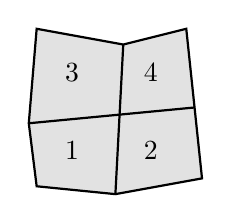
\begin{tikzpicture}
\draw[thick,fill=gray!23] (0,0)--(1,-0.1)--(2.1,0.1)--(1.9,2)--(1.1,1.8)--(0,2)--(-0.1,0.8)--cycle;  
\draw[thick] (-0.1,0.8)--(2,1);  
\draw[thick] (1,-0.1)--(1.1,1.8);  
\node[] at (0.45,0.45) {1};
\node[] at (1.45,0.45) {2};
\node[] at (0.45,1.45) {3};
\node[] at (1.45,1.45) {4};
\end{tikzpicture}




\end{center}
the corresponding matrix is given by\footnote{I suspect it should involve the normal vectors to the edges ...?}
\[
\tilde{h}
\left(
\begin{array}{cccc}
h_{12}+h_{13} & -h_{12} & -h_{13} & 0\\
-h_{12} & h_{12}+h_{24} & 0 & -h_{24} \\
-h_{13} & 0 & h_{13}+h_{34} & -h_{34} \\
0 & -h_{24} & -h_{34} & h_{24} + h_{34}
\end{array}
\right)
\left(
\begin{array}{c}
p_1 \\ p_2 \\ p_3 \\ p_4
\end{array}
\right)
\]
where $h_{ij}$ is the length/surface of the edge betweens elements $i$ and $j$. The reference length $\tilde{h}$ may be computed by simply defining it to be the average diameter of the constituent elements.


\begin{remark}
In three dimensions, the $2\times 2 \times 2$ block is the obvious starting point for stabilising $Q_1\times P_0$ \cite{grsa}.
\end{remark}


Perhaps the most serious potential drawback of the local framework is that stability is only guaranteed if the stabilisation parameter $\beta$ is bigger than some critical value $\beta_0$, which needs to be estimated.

It can be estimated that $\beta=1/4$ in 2D and $\beta=1/6$ in 3D (see Gresho \& Sani \cite[p636]{grsa} for a detailed derivation, see also \textcite{vibo92} (1992)).

Silvester \& Kechkar state: ``
The advantages of the stabilisation procedures over the penalty method
are especially relevant to the discretisation of 3D incompressible flow problems, since iterative solution methods have to be used.
Similar stabilisation techniques to those described here are applicable to the three-dimensional version of the $Q_1 \times P_0$ mixed method
''.

The conclusion in \cite{sike90} is as follows:
The local jump formulation proves to be an efficient method for a priori filtering of spurious pressure modes. It cleanly stabilises the $Q_1\times P_0$ mixed method without compromising
its simplicity and resulting efficiency; in particular, it is very robust with respect to the magnitude of the stabilisation parameter.

It is reported in Gresho \& Sani \cite{grsa} that when using an iterative solver, iteration counts
are only independent of the grid in the stabilised cases: using the raw $Q_1\times P_0$ method the iteration counts significantly increase with decreasing $h$. Note that the deterioration of the condition number of the matrix with decreasing $h$ is worse in 3D than in 2D (but
bear in mind that one almost always use higher resolutions in 2D than in 3D, so it does not help). 3D is also discussed in \cite{chsu97}.

A way to look at the global vs. local stabilisation schemes is presented
on the following figure from Christon (2002) \cite{chri02}:

\begin{center}
\includegraphics[width=10cm]{images/q1p0stab/chri02}\\
{\captionfont Element configuration for pressure stabilization: (a) global jump; (b) local jump.}
\end{center}

\begin{remark}
The locally stabilised Q1P0 and P1P0 elements have been analysed in Kechkar \& Silvester \cite{kesi92}. Penalty, global and local approaches are mentioned in Vincent \& Boyer (1992) but only the local jump
stabilisation is used. 
\end{remark}

Silvester (1994) investigates the value for $\beta$ for Q1P0 and 
arrives at $0.0615 \leq \beta \le 0.25$.
Chang \& Sugiyama (1997) report that ``a value between 0.01 and 0.1 appears to work well for most applications conducted so far''.
In \cite{elsw} the authors state that $\beta=\frac14$ is an idea value which ``ensures stability independently of the rectangle aspect ratio''.

Norburn \& Silvester (1998) state: ``Although the ‘optimal parameter’ (the value of $\beta$ which minimises the discretisation error on a given mesh) is impossible to determine a priori, good parameter choices (usually over-estimating the optimal parameter) can be
found by minimising the condition number of the pressure Schur complement matrix. [...]
The motivation for choosing the parameter value $\beta$ which minimises the condition number (ratio of largest to smallest eigenvalue) of the pressure Schur complement is that this quantity roughly determines the rate of convergence of Uzawa type iteration methods.'' They conclude that $\beta \simeq 0.1$ is appropriate for P1P0.

Rather interestingly we see that choosing the 'best' $\beta$ is primarily based in the literature on the Schur complement condition number, and less on the accuracy of the solutions (although it is sometimes assessed, see Fig.~4 of \textcite{nosi98} (1998)). 

Finally it is worth mentioning a recent paper by \textcite{chke20} (2020) who present modified 
local jump stabilisation schemes which effectively 
only take 2 or 1 one pressure jump into account instead
of 4 per macro-element. 

\vspace{.5cm}
%..............................................
In  three dimensions the matrix $\SSS$ is obtained by assembling the submatrices 
for the macroelements which, in general, are made up of 8 (i.e., $2\times 2 \times 2$) 
adjacent elements, as shown in the following sketch \cite{chsu97}:

\begin{center}
\includegraphics[width=4cm]{images/q1p0stab/macro3D}\\
{\captionfont Numbering of hexahedrons in a macroelement.\\ 
Element No. 3 is behind No. 1 and below No. 7.} 
\end{center}

For a macroelement of 8 elements as ordered in the above sketch, the submatrix is defined below:

\[
\SSS=
\left(
\begin{array}{cccccccc}
h_{12}+h_{13}+h_{h15} & -h_{12} & -h_{13} &  0  &  -h_{15} & 0  & 0 & 0 \\
-h_{21} & h_{21}+h_{24} + h_{26} & 0 & -h_{24} & 0 & -h_{26} & 0 & 0 \\
-h_{31} & ... \\
0 & ... \\
-h_{51} & ...\\
0 & ...\\
0 & ...\\
0 & ...
\end{array}
\right)
\]
in which $h_{ij}$ is the length scale for elements `i' and `j' in the macroelement. 
The matrix $\SSS$ is symmetric, since $h_{ij}=h_{ji}$. 

Two approaches are possible  for computing the length scale $h_{ij}$:
\begin{itemize}
\item the square root of the interior inter-element surface area between elements `i' and `j' 
\item the quotient of the interior inter-element surface area divided by the cube 
root of the average element volume of the macroelement.
\end{itemize}


\vspace{.5cm}

%%%%%%%%%%%%%%%%%%%%%%%%%%%%%%%%%%%%%%%%%%
\paragraph{Macro-element}

One source for this stabilisation approach is Section~5.3.2 of the book by Elman, Silvester and Wathen \cite{elsw}.
The $\C$ matrix for the 2D macroelement is shown to be:
\[
\C = \beta
\left(
\begin{array}{cccc}
1 &-1& 1 &-1 \\
-1& 1& -1& 1 \\
1 &-1& 1 &-1 \\
-1& 1& -1& 1 
\end{array}
\right)
\]
and the authors suggest $\beta = \frac14 h_xh_y$.  

\input{tikz/tikz_q1p0stab_macro}

Also see \cite{fobo90} (1990) .

\vspace{.5cm}
%\newpage
%%%%%%%%%%%%%%%%%%%%%%%%%%%%%%%%%%%%%%%%%%%%%%%%%%%%%%%
\paragraph{Numerical scaling of $\C$}

Since the matrix $\mathbb{K}$ contains the viscosity, it is to be expected that the magnitude of the entries in matrix $\mathbb{C}$ must somehow follows the values in the $\mathbb{G}^T \cdot \mathbb{K}^{-1} \cdot \mathbb{G}$  term. Indeed the Schur complement is $\G^T\cdot\K^{-1}\cdot\G+\C$ so if the entries in $\C$ are wrongly scaled it will either have no effect at all or will alter the solution too much.
This is indeed what is advocated in Christon (2002) \cite{chri02}:

\begin{center}
\includegraphics[width=10cm]{images/q1p0stab/chri02a}\\
{\captionfont In the paper $S$ stands for $\C$, and $C$ stands for $\G$. Also, because Christon is solving the N-S equations,\\ and because of his algorithmic choice to do so, there is a velocity mass matrix where our $\K$ block resides. As such\\ his implementation showcases the lumped mass matrix in the equation above rather than the lumped $\K$ matrix.\\} 
\end{center}

In the paper Christon states that the PPE term $C^TM_L^{-1}C$
is symmetric. This is obviously true since it is a scalar for the $Q_1\times P_0$ element. Am I missing something here?

Using our notations, the off-diagonal entries of the stabilisation matrix $\C$ for the global approach  becomes:
\begin{equation}
\C_{ef} = -\beta (\G^T\cdot \K_L^{-1} \cdot \G)_{e} 
\frac{1}{\Gamma_{ef}} \int_{\Gamma_{ef}} \llbracket \psi_e \rrbracket \; \llbracket \psi_f \rrbracket d\Gamma
\qquad
\text{for} \; e\ne f
\label{eq:Cchriston}
\end{equation}
where $e$ and $f$ identify adjacent elements that share a common face, $\Gamma_{ef}$ represents the shared inter-element boundary (a length in 2D, a surface in 3D),  $\beta$ is a non-dimensional scaling parameter, and $\K_L$ is the row-wise lumped $\K$ matrix\footnote{
The quantity $\mathbb{G}^T \cdot \mathbb{K}^{-1} \cdot \mathbb{G}$ for $Q_1\times P_0$ elements is a scalar,
which is rather convenient as it gives in a simple way the scaling for the stabilisation term. However the inverse of $\K$ is costly so there is a cheaper alternative which consists in lumping it so that it becomes diagonal and its inverse is then trivial.}.
For the $Q_1\times P_0$ element, the pressure approximation is piecewise constant with $\psi_i=1$ inside the element and zero outside.

The inclusion of the $\G^T\cdot \K_L^{-1} \cdot \G$
term  in the stabilisation yields proper dimensionality of the stabilization matrix (the integrand is dimensionless so that the dimensions of $\C$ are those of the elemental Schur complement block), accounts for scaling due to irregular elements, and still preserves the symmetry \cite{chri02}.


Finally, the diagonal element of $C$ for element $e$ is computed as 
\[
\C_{ee} =  \beta (\G^T\cdot \K_L^{-1} \cdot \G)_{e} 
\sum_{f\ne e} \frac{1}{\Gamma_{ef}} \int_{\Gamma_{ef}} \llbracket \psi_e \rrbracket \; \llbracket \psi_f \rrbracket d\Gamma
\]
We find that the sum of the terms on the row corresponding to $e$ is indeed zero, consistency is ensured even for non-rectangular elements.

There is however a major problem with this approach: even when the viscosity is constant in the domain, Eq.~\eqref{eq:Cchriston} does not yield a symmetric matrix if elements are not identical in shape. 
Since $\C_{ef} \propto (\G^T\cdot \K_L^{-1} \cdot \G)_{e}$
then $\C_{ef} \neq \C_{fe}$!
I then suspect that Christon's notation $|C^TM_L^{-1}C|_{IJ}$
indicates that some care must be taken so as to ensure $S_{IJ}=S_{JI}$ but it is not further specified.
We will then have to figure this out. 

\vspace{.5cm}


Let us consider the case of square elements of size $h_x=h_y=h$. Then the $\K_e$ and $\G_e$ matrices are given by:
\[
\K_e=
\left(
\begin{array}{cccccccc}
1    & 0.25 & -0.5 & -0.25 & -0.5  & -0.25 & 0     & 0.25 \\
0.25 & 1    & 0.25 & 0     & -0.25 & -0.5  & -0.25 & -0.5 \\
-0.5 & 0.25 & 1    & -0.25 &     0 & -0.25 & - 0.5 & 0.25 \\
-0.25 & 0 & -0.25 & 1 & 0.25 & -0.5 & 0.25 & -0.5 \\
-0.5 & -0.25 & 0 & 0.25 & 1 & 0.25 & -0.5 & -0.25 \\
-0.25 & -0.5 & -0.25 & -0.5 & 0.25 & 1 & 0.25 & 0 \\
0 & -0.25 & -0.5 & 0.25 & -0.5 & 0.25 & 1 & -0.25 \\
0.25 & -0.5 & 0.25 & -0.5 & -0.25 & 0 & -0.25 & 1 
\end{array}
\right)
\qquad 
\G_e=h
\left(
\begin{array}{c}
+1/2\\
+1/2\\
-1/2\\
+1/2\\
-1/2\\
-1/2\\
+1/2\\
-1/2
\end{array}
\right)
\]
so that the Schur complement is 
\[
\SSS_e = \G^T_e \cdot \tilde{\K}_e^{-1} \cdot \G_e
= \frac{2}{3}h^2
\]
In that case we almost recover the expression of for example the macro-element. 


\vspace{.5cm}

%%%%%%%%%%%%%%%%%%%%%%%%%%%%%%%%%%%%%%%%%%%%%%%%%%%%%%%%%%
\paragraph{Dealing with viscosity contrasts/large variations}


This topic is almost never discussed as many papers consider
the standard Stokes equations with $\eta=1$ (and also regular meshes made of identical elements). This is not 
problematic in engineering where often the fluid in question 
has a constant viscosity (or the equations have been rendered dimensionless). However, in geodynamical applications
we know that the viscosity field can showcase very sharp gradients (sinking/rising objects, shear bands, free surface, ...). In what follows we assume that each element $e$ has an effective viscosity $\eta_e$. 

The scaling of the $\C$ matrix in the previous section is not formulated when viscosity contrasts from one element to the other are present. For example scaling the row entries of the $\C$ matrix by the element viscosity still yields a structurally symmetric matrix, but not a numerically symmetric one which is problematic since we have seen that $\C$ must be semi-positive definite. Some form of viscosity averaging must then take place between adjacent elements so that the contribution from element $e$ to $ f$ is exactly the same as $f$ to $e$

In order for the stabilisation to remain consistent it must satisfy $\C\cdot \vec{1}= 0$, i.e. it should have zero effect on a constant pressure field, which then forces the sum of the entries for each row (or column) to be null. This requirement makes the above viscosity averaging idea very difficult in practice in the global case (satisfying both symmetry and consistency).

%One could then decide to use a reference viscosity valid for the whole domain which would provide adequate (numerical) scaling but not account for viscosity contrasts.

%In the previous section we have $\C \propto (\G^T\cdot \K_L^{-1} \cdot \G)_{e} $ which is problematic since it is not symmetric.
%Once again, Christon uses a double subscript on this term but does not explain what it means.  

Let us start by defining the elemental Schur complement
\[
\tilde{\SSS}_e = |(\G^T\cdot \K_L^{-1} \cdot \G)_e|
\]
and then 
\[
\tilde{\SSS}_{ef} = \phi( \tilde{\SSS}_e , \tilde{\SSS}_f)   
\]
where $\phi$ is a function to be specified later such that $\phi(x,y)=\phi(y,x)$.
The local and global jump stabilisation can then be 
formulated as follows:
\begin{equation}
\C_{ef} = -\beta \tilde{\SSS}_{ef}  
\frac{1}{\Gamma_{ef}} \int_{\Gamma_{ef}} \llbracket \psi_e \rrbracket \; \llbracket \psi_f \rrbracket d\Gamma
\qquad
\text{for} \; e\ne f
\label{eq:Cchriston2}
\end{equation}
supplemented by
\[
\C_{ee} =  \beta 
\sum_{f\ne e} \tilde{\SSS}_{ef}\frac{1}{\Gamma_{ef}} \int_{\Gamma_{ef}} \llbracket \psi_e \rrbracket \; \llbracket \psi_f \rrbracket d\Gamma
\]
In this case the matrix $\C$ is symmetric and consistent!



\newpage
%%%%%%%%%%%%%%%%%%%%%%%%%%%%%%%%%%%%%%%%%%%%%%%%%%%%%%
\paragraph{Recap}: For each element compute its (scalar) Schur complement
\[
\tilde{\SSS}_e = |(\G_e^T\cdot \tilde{\K}_e^{-1} \cdot \G)|
\]
We here assume that elements can have different viscosities and/or shape so that $\SSS_e$ varies 
from element to element. 

\begin{itemize}
\item{Global jump} Assuming elements $e$ and $f$ share and edge, build the $\C$ matrix as follows:
\begin{equation}
\C_{ef} = -\beta \tilde{\SSS}_{ef}  
\frac{1}{\Gamma_{ef}} \int_{\Gamma_{ef}} \llbracket \psi_e \rrbracket \; \llbracket \psi_f \rrbracket d\Gamma
\qquad
\text{for} \; e\ne f
\end{equation}
supplemented by
\[
\C_{ee} =  \beta 
\sum_{f\ne e} \tilde{\SSS}_{ef}\frac{1}{\Gamma_{ef}} \int_{\Gamma_{ef}} \llbracket \psi_e \rrbracket \; \llbracket \psi_f \rrbracket d\Gamma
\]

\item{Local jump}  Let ${\cal M}_e$ be the macroelement that element $e$ is in. Assuming elements $e$ and $f$ share and edge, build the $\C$ matrix as follows:
\begin{equation}
\C_{ef} = -\beta \tilde{\SSS}_{ef}  
\frac{1}{\Gamma_{ef}} \int_{\Gamma_{ef}} \llbracket \psi_e \rrbracket \; \llbracket \psi_f \rrbracket d\Gamma
\qquad
\text{for} \; e\ne f \quad \text{and} \quad f\in {\cal M}_e
\end{equation}
supplemented by
\[
\C_{ee} =  \beta 
\sum_{f\ne e, f\in {\cal M}_e} \tilde{\SSS}_{ef}\frac{1}{\Gamma_{ef}} \int_{\Gamma_{ef}} \llbracket \psi_e \rrbracket \; \llbracket \psi_f \rrbracket d\Gamma
\]



\item{Macroelement stab} 
Let ${\cal M}_e$ be the macroelement that element $e$ is in. 
\begin{center}
\begin{flushright} {\tiny {\color{gray} (tikz\_macro2.tex)}} \end{flushright}
%~~~~~~~~~~~~~~~~~~~~~~~~~~~~~~~~~~~~~~~~~~~~~~~~~~~~~~~~~~~~~~~~~~~~~~~~~~~~~~~~~~~~~~~~~~~~~~~~~~


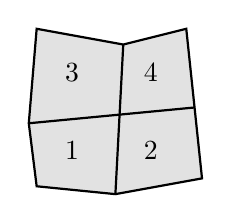
\begin{tikzpicture}
\draw[thick,fill=gray!23] (0,0)--(1,-0.1)--(2.1,0.1)--(1.9,2)--(1.1,1.8)--(0,2)--(-0.1,0.8)--cycle;  
\draw[thick] (-0.1,0.8)--(2,1);  
\draw[thick] (1,-0.1)--(1.1,1.8);  
\node[] at (0.45,0.45) {1};
\node[] at (1.45,0.45) {2};
\node[] at (0.45,1.45) {3};
\node[] at (1.45,1.45) {4};
\end{tikzpicture}




\end{center}

This is less straighforward than the local jump since 
(for example) elements 1 and 4 do not have an edge in common so that the jump operator cannot be used. 
One could think of assigning all four elements a single effective viscosity but elements shapes/sizes can differ and the matrix is then not necessarily consistent. 
One should probably go back to the derivations in 
\textcite{elsw} and see whether a more generic form of the macroelement stabilisation matrix $\C$ could be derived?

\end{itemize}

